\chapter{Linear Gaussian Systems}
\label{chapter:linear_gaussian}

The following three conditions are sufficient, in addition to the Markov assumption, to ensure that the belief, $p \left( \pmb{x}_{t} \right)$, of the system is always Gaussian~\cite{Thrun_rec, Thrun_gauss}:

\begin{enumerate}
\item The state transition probability $p(\pmb{x}_{t} | \pmb{x}_{t-1}, \pmb{u}_{t})$ is a linear function in its arguments, with added Gaussian noise.
\begin{align}
\pmb{x}_{t} &= A_{t} \pmb{x}_{t-1} + B_{t} \pmb{u}_{t} + \pmb{\epsilon}_{t}
\end{align}
$A_{t}$ and $B_{t}$ are $n \times n$ and $m \times n$ matrices respectively, with $n$ being the dimension of the sate vector. $\pmb{\epsilon}_t$ is a Gaussian random vector which accounts for the uncertainty introduced during state transition, it is zero mean with a covariance matrix $R_{t}$. The state transition probability is now given as:
\begin{align*}
& p(\pmb{x}_{t} | \pmb{x}_{t-1}, \pmb{u}_{t}) = \mathcal{N} \left( \pmb{x}_{t} | A \pmb{x}_{t-1} + B \pmb{u}_{t}, R_{t} \right) \\
&= \frac{1}{ (2 \pi)^{n/2} |R|^{1/2} } \exp{\left\{ -\frac{1}{2} \left( \pmb{x}_{t} - A_{t} \pmb{x}_{t-1} + B \pmb{u}_{t} \right)^{T} R_{t}^{-1} \left( \pmb{x}_{t} - A_{t} \pmb{x}_{t-1} + B \pmb{u}_{t} \right) \right\} } \label{eqn:trans_prob} \numberthis
\end{align*}
\item The measurement probability, $p \left( \pmb{z}_{t} | \pmb{x}_{t} \right)$, must also be linear in its arguments, with added Gaussian Noise:
\begin{align}
\pmb{z}_{t} &= C_{t} \pmb{x}_{t} + \pmb{\delta}_{t}
\end{align}
$C_{t}$ is $k \times n$ matrix, $\pmb{z}_{t}$ being $k$ dimensional. $\pmb{\delta}_{t}$ is zero mean Gaussian noise with a covariance of $Q_{t}$. $p \left( \pmb{z}_{t} | \pmb{x}_{t} \right)$ is now defined as:
\begin{align*}
& p(\pmb{z}_{t} | \pmb{x}_{t}) = \mathcal{N} \left( \pmb{z}_{t} | C_{t} \pmb{x}_{t}, Q_{t} \right) \\
&= \frac{1}{ (2 \pi)^{k/2}|Q|^{1/2} } \exp{\left\{ -\frac{1}{2} \left( \pmb{x}_{t} - C_{t} \pmb{x}_{t} \right)^{T} Q_{t}^{-1} \left( \pmb{z}_{t} - C_{t} \pmb{x}_{t}\right) \right\} } \label{eqn:mes_prob}  \numberthis
\end{align*}
\item The belief about the initial state, $p \left( \pmb{x}_{0} \right)$, must be normally distributed:
\begin{align*}
& p(\pmb{z}_{t} | \pmb{x}_{t}) = \mathcal{N} \left( \pmb{x}_{0} | \pmb{\mu}_{t} , \Sigma_{t} \right) \\
\end{align*}
\end{enumerate}
\begin{remark}
This entire section was shamelessly stolen from~\cite{Thrun_gauss}, but it's necessary to restate all of this to establish the ground rules and introduce some notation. The notation quickly becomes an unbearable mess from this point onwards.
\end{remark}

\section{Bayes Net Representation}
\label{section:bayes_net}
\begin{definition}[Bayesian Network]
A Bayesian Network is a distribution of the form:
\begin{align}
p\left(\pmb{x}_{1}, \cdots, \pmb{x}_{N}\right) &= p\left(\pmb{x}^{N}_{0} \right) = \prod^{N}_{i=1} p\left(x_{i} | \mbox{pa} (\pmb{x}_{i}) \right)
\label{eqn:bayes_net_def}
\end{align}
where $\mbox{pa} \left( x_{i} \right) $ are the \textbf{parental} variables of $x_{i}$. It is represented naturally as a directed graph, with a directed edge from the parent to its child. The $j^{th}$ node corresponds to the factor $p\left(\pmb{x}_{j} | \mbox{pa} (\pmb{x}_{j}) \right)$~\cite{Koller_bayes_net, Barber_belief_net}.
\end{definition}
The Kalman Filter can be represented as a joint density function of all random variables $\pmb{x}^{t}_{0}$ and $\pmb{z}^{t}_{1}$, without any loss of generality\footnote{Okay, I'm not sure if this is true, but I've always wanted to say it.}. This allows the following factorisation:
\begin{align*}
p \left( \pmb{x}_{0}^{t}, \pmb{z}_{1}^{t}, \pmb{u}_{1}^{t} \right) &= p\left( \pmb{z}_{t} | \pmb{x}_{t}, \pmb{z}_{1}^{t-1}, \pmb{u}_{1}^{t} \right) p \left( \pmb{x}_{0}^{t}, \pmb{z}_{1}^{t-1}, \pmb{u}_{1}^{t} \right) \\
&= p\left( \pmb{z}_{t} | \pmb{x}_{t}, \pmb{z}_{1}^{t-1}, \pmb{u}_{1}^{t}\right) p \left( \pmb{x}_{0}^{t} | \pmb{x}_{0}^{t-1},  \pmb{z}_{1}^{t-1}, \pmb{u}_{1}^{t} \right) p \left( \pmb{x}_{0}^{t-1}, \pmb{z}_{1}^{t-1}, \pmb{u}_{1}^{t-1} \right) \label{eqn:bayes_rec} \numberthis
\end{align*}
Applying the Markov assumption to Equation~\ref{eqn:bayes_rec} and then following the recursion to its conclusion, results in:
\begin{align}
p \left( \pmb{x}_{0}^{t}, \pmb{z}_{1}^{t}, \pmb{u}_{1}^{t} \right) &= p \left( \pmb{x}_{0} \right) \prod^{t}_{i=1} p \left( \pmb{z}_{i} | \pmb{x}_{i} \right) p \left( \pmb{x}_{i} | \pmb{x}_{i-1}, \pmb{u}_{t} \right) \label{eqn:kalman_factor}
\end{align}
The form of Equation~\ref{eqn:kalman_factor} is exactly that of Equation~\ref{eqn:bayes_net_def} allowing the Kalman Filter to be represented naturally as a Bayes Net, as seen in Figure~\ref{figure:bayes_net}. 
\begin{remark}
The representation of Equation~\ref{eqn:kalman_factor} is misleading. The control vector, $\pmb{u}_{t}$, is not a random variable, it is deterministic and known in each state. 
\end{remark}


\documentclass[tikz]{standalone}
\usepackage{amsfonts}
\usepackage{amsmath}
\usepackage{amssymb}
\usepackage{tikz}
\begin{document}

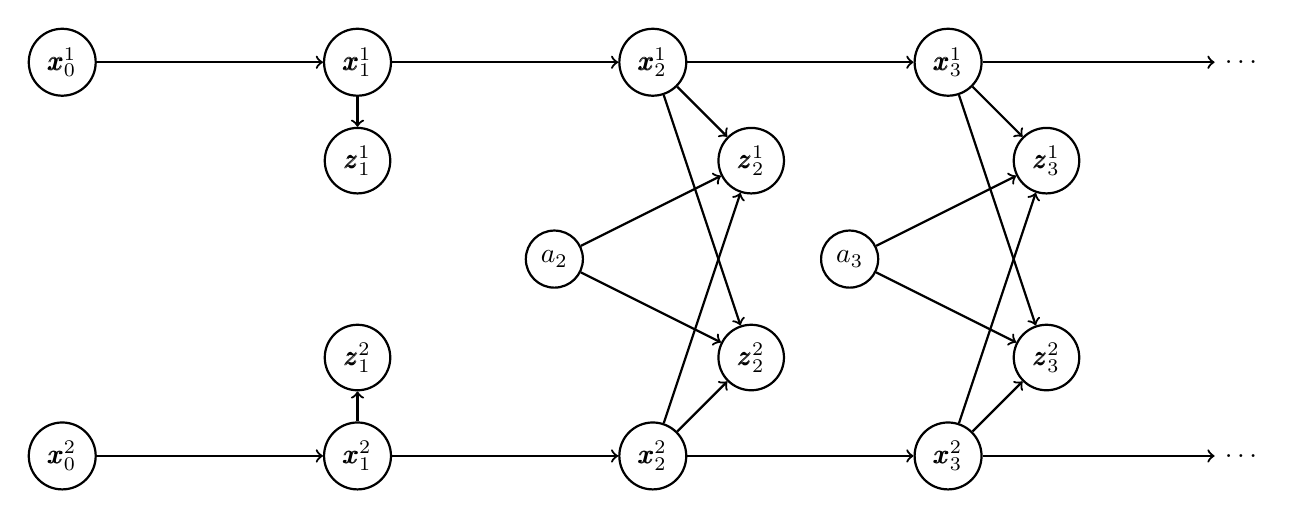
\begin{tikzpicture}

\begin{scope}[every node/.style={circle,thick,draw}]
	%Frame 1
	\node (x_0^1) at (-3.75, 0) {$\pmb{x}_{0}^{1}$};
	\node (x_0^2) at (-3.75, -5) {$\pmb{x}_{0}^{2}$};
	
	%Frame 2
	\node (x_1^1) at (0, 0) {$\pmb{x}_{1}^{1}$};
	\node (z_1^1) at (0, -1.25) {$\pmb{z}_{1}^{1}$};
	
	\node (z_1^2) at (0, -3.75) {$\pmb{z}_{1}^{2}$};
	\node (x_1^2) at (0, -5) {$\pmb{x}_{1}^{2}$};
	
	%Frame 3
	\node (x_2^1) at (3.75, 0) {$\pmb{x}_{2}^{1}$};
	
	\node (a_2) at (2.5, -2.5) {$a_{2}$};
	\node (z_2^1) at (5, -1.25) {$\pmb{z}_{2}^{1}$};
	\node (z_2^2) at (5, -3.75) {$\pmb{z}_{2}^{2}$};
	
	\node (x_2^2) at (3.75, -5) {$\pmb{x}_{2}^{2}$};
	
	%Frame 4
	\node (x_3^1) at (7.5, 0) {$\pmb{x}_{3}^{1}$};
	
	\node (a_3) at (6.25, -2.5) {$a_{3}$};
	\node (z_3^1) at (8.75, -1.25) {$\pmb{z}_{3}^{1}$};
	\node (z_3^2) at (8.75, -3.75) {$\pmb{z}_{3}^{2}$};
	
	\node (x_3^2) at (7.5, -5) {$\pmb{x}_{3}^{2}$};
\end{scope}

\begin{scope}[style={thick,draw}]
	%Frame 5
    \node (xdot1) at (11.25, 0) {\dots};
    \node (xdot2) at (11.25, -5) {\dots};
\end{scope}

\begin{scope}[style={thick,draw}]
	%Frame 1
	\path [->] (x_0^1) edge node {} (x_1^1);
	\path [->] (x_0^2) edge node {} (x_1^2);
	
	%Frame 2
	\path [->] (x_1^1) edge node {} (x_2^1);
	\path [->] (x_1^1) edge node {} (z_1^1);
	
	\path [->] (x_1^2) edge node {} (z_1^2);
	\path [->] (x_1^2) edge node {} (x_2^2);

	%Frame 3
	\path [->] (x_2^1) edge node {} (x_3^1);
	\path [->] (x_2^1) edge node {} (z_2^1);
	\path [->] (x_2^1) edge node {} (z_2^2);
	
	\path [->] (a_2) edge node {} (z_2^1);
	\path [->] (a_2) edge node {} (z_2^2);
	
	\path [->] (x_2^2) edge node {} (x_3^2);
	\path [->] (x_2^2) edge node {} (z_2^1);
	\path [->] (x_2^2) edge node {} (z_2^2);
		
	%Frame 4
	\path [->] (x_3^1) edge node {} (xdot1);
	\path [->] (x_3^1) edge node {} (z_3^1);
	\path [->] (x_3^1) edge node {} (z_3^2);
	
	\path [->] (a_3) edge node {} (z_3^1);
	\path [->] (a_3) edge node {} (z_3^2);
	
	\path [->] (x_3^2) edge node {} (z_3^1);
	\path [->] (x_3^2) edge node {} (z_3^2);
	\path [->] (x_3^2) edge node {} (xdot2);
\end{scope}

\end{tikzpicture}

\end{document}

\section{Junction Tree Representation}
\label{section:cluster_graph}
The Junction Tree Algorithm is a form of tree decomposition which seeks to eliminate cycles in a graph by clustering them into a single node. With the cycles removed  it is possible to perform exact inference, avoiding any iterative message passing schemes.

\begin{remark}
I was going to define clusters graphs, the generalised running intersection property and then arrive at clique trees, but it seemed daunting. Also pointless, considering I'm the only person who will ever read this and any definitions I give will just be rehashed versions of those given by Koller and Barber.
\end{remark}


\subsection{Junction Tree Construction: The HUGIN Algorithm}
\label{subsection:jtree_construction}
The HUGIN algorithm provides a procedure for constructing a Junction tree from some general graph~\cite{Du_Preez_week5}:

\begin{enumerate}
\item If the graph if directed, moralize it. Moralization will produce the equivalent undirected form of the graph, preserving the underlying probabilistic dependencies.
\item Triangulate the graph using variable elimination, this will produce the induced graph. Elimination ordering determines the density of the induced graph, an ordering is sought which will introduce the least amount of fill edges.
\item Identify all maximal cliques in the induced graph, the variables in cliques are then assigned to this \textit{supernode}.
\item Allocate each potential from the original graph to exactly one of these \textit{super} nodes. The \textit{supernode} is simply a product of all of its associated potentials.
\item Find a maximal spanning tree over all the \textit{supernodes}.
\end{enumerate}

\subsubsection{Application to the Kalman Filter}
\label{section:kalman_filter}
The Kalman Filter's Bayes Net representation is already a tree, therefore its decomposition is trivial. Moralization introduces no new edges as all child nodes only have a single parent. The variable elimination orderings are also trivial, the leaf nodes can eliminated in any order and will also introduce no fill edges into the induced graph. The remaining chain structure only has two possible elimination orderings, forwards or backwards, both are perfect and introduce no fill edges. All maximal cliques comprise of a adjacent parings of nodes, which only need to assigned a single potential. The maximal spanning tree is the existing tree as sepsets are single variable sets, $\pmb{S}_{i, j} = \pmb{C}_{i} \cap \pmb{C}_{j} = \{ \pmb{x}_{i} \} $.

The Junction Tree equivalent of Figure~\ref{figure:bayes_net} can be seen in Figure~\ref{figure:junction_tree}.

\begin{figure}
\centering
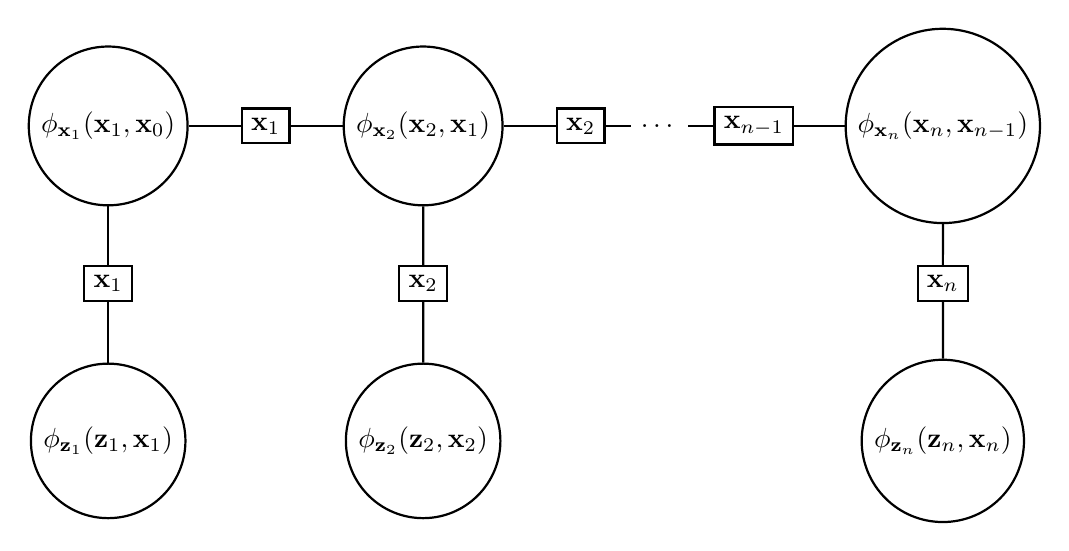
\begin{tikzpicture}[scale=0.80]
\begin{scope}[every node/.style={circle,thick,draw}]
    \node (x1) at (0, 0) {$\phi_{\mathbf{x}_1} (\mathbf{x}_{1}, \mathbf{x}_{0})$};
    \node (z1) at (0, -5) {$\phi_{\mathbf{z}_1} (\mathbf{z}_{1}, \mathbf{x}_{1})$};

    \node (x2) at (5, 0) {$\phi_{\mathbf{x}_2} (\mathbf{x}_{2}, \mathbf{x}_{1})$};
    \node (z2) at (5, -5) {$\phi_{\mathbf{z}_2} (\mathbf{z}_{2}, \mathbf{x}_{2})$};
    
    \node (xn) at (13.25, 0) {$\phi_{\mathbf{x}_n} (\mathbf{x}_{n}, \mathbf{x}_{n-1})$};
    \node (zn) at (13.25, -5) {$\phi_{\mathbf{z}_n} (\mathbf{z}_{n}, \mathbf{x}_{n})$};

\end{scope}

\begin{scope}[every node/.style={thick,draw}]
    \node (sz1) at (0, -2.5) {$\mathbf{x}_{1}$};
    \node (sx1) at (2.5, 0) {$\mathbf{x}_{1}$};
    
    \node (sz2) at (5, -2.5) {$\mathbf{x}_{2}$};
    \node (sx2) at (7.5, 0) {$\mathbf{x}_{2}$};
    
    \node (sxn) at (10.25,0) {$\mathbf{x}_{n-1}$};
    \node (szn) at (13.25, -2.5) {$\mathbf{x}_{n}$};
\end{scope}

\begin{scope}[style={thick,draw}]
    \node (xdot1) at (8.75,0) {\dots};
\end{scope}


\begin{scope}[style={thick,draw}]
	\path [-] (x1) edge node {} (sz1);
	\path [-] (sz1) edge node {} (z1);
	\path [-] (x1) edge node {} (sx1);
	\path [-] (sx1) edge node {} (x2);
	
	\path [-] (x2) edge node {} (sz2);
	\path [-] (sz2) edge node {} (z2);
	\path [-] (x2) edge node {} (sx2);
	\path [-] (sx2) edge node {} (xdot1);

	\path [-] (xdot1) edge node {} (sxn);	
	\path [-] (sxn) edge node {} (xn);
	\path [-] (xn) edge node {} (szn);	
	\path [-] (szn) edge node {} (zn);
	
\end{scope}

\end{tikzpicture}

\caption[Equivalent Junction Tree for a Kalman Filter.]{The junction tree  resulting  from the Bayes Net in Figure~\ref{figure:bayes_net}.}
\label{figure:junction_tree}
\end{figure}

\subsection{Message Passing: Integral-Product Algorithm}
\label{subsection:message_passing}
 
\begin{definition} [Integral-Product Message Passing] \label{def:int_prod}
In a cluster graph, $\mathcal{T}$, defined for a set of continuous factors $\Phi$ over $\mathcal{X}$, the message from a cluster $\pmb{C}_{i}$ to an adjacent cluster $\pmb{C}_{j}$ is computed using the \textbf{integral-product message passing} computation:
\begin{align}
\delta_{i \rightarrow j} &= \int \psi_{i} \left( \prod_{k \in \left( \mbox{Nb}_{i} - \{ j \} \right)} \delta_{k \rightarrow i} \right) d\{ {\pmb{C}_{i} - \pmb{S}_{i, j}} \} \label{eqn:int_prod}
\end{align}
Here $\psi_{i}$ is the potential assigned to $\pmb{C}_{i}$ and $\mbox{Nb}_{i}$ are all clusters adjacent to it~\cite{Barber_junction_tree, Koller_clique_trees, Koller_canonical}.
\end{definition}
From Definition~\ref{def:int_prod} it can be seen that the Junction Tree algorithm does not necessarily simplify inference, with its larger nodes the work of iterative message passing is simply shifted to this integral.


